\documentclass[conference]{IEEEtran}
\IEEEoverridecommandlockouts
% The preceding line is only needed to identify funding in the first footnote. If that is unneeded, please comment it out.
%Template version as of 6/27/2024

\usepackage{cite}
\usepackage{amsmath,amssymb,amsfonts}
\usepackage{algorithmic}
\usepackage{graphicx}
\usepackage{textcomp}
\usepackage{xcolor}
\usepackage{hyperref}
\usepackage{array}
\usepackage{arydshln}
\usepackage{multicol}
\usepackage{wrapfig}
\usepackage{listings}
\usepackage{subfig}
\usepackage{graphicx,subcaption,lipsum}
\newcolumntype{P}[1]{>{\centering\arraybackslash}p{#1}}
\newcolumntype{M}[1]{>{\centering\arraybackslash}m{#1}}


\begin{document}

\title{3D Vehicle Reconstruction via Monocular Camera with Deep Learning Models and Direct Linear Transformation\\
{\footnotesize 2024-2 Robot Vision (M3228.003000)}
}

\author{
    \IEEEauthorblockN{Thomas Putzer}
    \IEEEauthorblockA{\textit{Computer Science and Engineering} \\
        \textit{Seoul National University}\\
        Seoul, South Korea \\
        putzerthomas55@gmail.com}
    \and
    \IEEEauthorblockN{Weihao Chao}
    \IEEEauthorblockA{\textit{Mechanical Engineering} \\
        \textit{Seoul National University}\\
        Seoul, South Korea \\
        theweihao@gmail.com}
    \and
    \IEEEauthorblockN{Anggraini Ditha}
    \IEEEauthorblockA{\textit{Civil and Environmental Engineering} \\
        \textit{Seoul National University}\\
        Seoul, South Korea \\
        dithanggraini1598@gmail.com}
}

\maketitle

\begin{abstract}
    Hello here goes the abstract
\end{abstract}

\section{Project Objectives}

This project aims to develop a workflow for reconstructing wireframe 3D vehicle models from monocular camera images. The approach involves detecting keypoints of vehicles using a deep learning framework, OpenPifPaf, that is designed for detecting human poses (key points) and other object structures within images. Using the CarFusion dataset (Reddy et al., 2018), we trained the deep learning model to recognize key vehicle features and use those to estimate a basic 3D model of vehicles and to estimate vehicle speed. 

Previous research in 3D vehicle reconstruction often relies heavily on deep learning models throughout the pipeline, utilizing techniques such as Graph Neural Networks (GNNs) in combination with Convolutional Neural Networks (CNNs) or transformers. While these methods can achieve high accuracy, they are computationally intensive and require substantial processing power, making them less practical for real-time applications or deployment on resource-constrained devices. Our project takes a different approach by limiting the use of deep learning to the initial stage of keypoint detection, where it excels at identifying critical features such as vehicle parts and keypoints from 2D images. Once these keypoints are identified, the methodology transitions to geometry-based point tracking and traditional computer vision techniques to perform 3D reconstruction and pose estimation. This strategic design significantly improves computational efficiency, as geometry-based methods are less resource-intensive than deep learning while still being capable of leveraging the spatial relationships inherent in 3D space. Our project also proposes the application of the RANSAC (Random Sample Consensus) algorithm for robust handling of errors in detected keypoints. Finally, while previous research focuses on static 3D pose reconstruction, our project extends its scope to estimate vehicle speed dynamically over time by utilizing primitive frame-by-frame car tracking
\ref{img:workflow}.

\begin{figure}
    \centering
    \includegraphics[width=0.9\columnwidth]{./images/workflow.png}
    \caption{Project workflow.}
    \label{img:workflow}
\end{figure}

\section{Vehicle Key Point Detection}

In this project, we adapt the OpenPifPaf pose-detection deep learning model for car keypoint detection. Using Carfusion datasets for testing and training data. For initial training, we utilized a pre-trained model with a ResNet-101 backbone. We trained the model on a subset of 10 images over 150 epochs. For this model, we successfully generated the weight file as well as the keypoint data of the predicted image.

\begin{figure}[h]
    \centering
    \subfloat[\centering label 1]{{\includegraphics[width=.48\columnwidth]{./images/keypoint_vis1.jpg} }}
    \subfloat[\centering label 2]{{\includegraphics[width=.48\columnwidth]{./images/keypoint_vis3.jpg} }}
    \caption{Examples of the predicted key points from the OpenPifPaf model. Detected keypoints are shown in yellow and the computed bounding box in red. The overall confidence score is shown above the bounding box.}
    \label{img:keypoints}
\end{figure}

\section{3D Pose Estimation}

\subsection{Geometry Processing}

To understand the 3d pose estimation process a basic understanding of the geometry processing stage of the 3d rendering pipeline is required. That is the process of how a 3d model and its vertices are transformed from points in 3d space to pixels on a 2d screen. 

The vertices of a 3D model are defined in their local coordinate system, the so-called local space. If the model is placed inside the 3D scene, its position in world space can be controlled with the model matrix $M_{mod}$. World space is the coordinate system of the \textit{world}, the 3d scene where all the objects, lights, and the camera live. The camera's position and rotation in world space are determined by the inverse of the view matrix $M_{view}^{-1}$. For the next steps of the 3D rendering pipeline, it is generally preferred to have objects in view space rather than world space. View space is the reference frame of the camera, meaning the camera is located at its origin looking straight ahead. To transform an object from world- into viewspace, it just needs to be multiplied by the view matrix, meaning to get from local- to view space the composition of the model and view matrices can be used: this composition is called model view Matrix $M_{MV}=M_{view}M_{mod}$.

The next step is figuring out where on the screen a vertex should be drawn. Once in view space, the projected position on the $z = 1$ plane can be computed by dividing the position of a vertex by its z-component. More formally you can multiply by the projection matrix and divide by the w-component. This matrix representation of the standard projection onto the $z = 1$ plane looks like this:

\begin{equation}
    \begin{bmatrix}
        1 & 0 & 0 & 0 \\
        0 & 1 & 0 & 0 \\
        0 & 0 & 1 & 0 \\
        0 & 0 & 1 & 0
    \end{bmatrix}
    \begin{bmatrix}
        x \\
        y \\
        z \\
        1
    \end{bmatrix}
    =
    \begin{bmatrix}
        x \\
        y \\
        z \\
        z
    \end{bmatrix}
    \overset{\text{div z}}{\equiv}
    \begin{bmatrix}
        \frac{x}{z} \\
        \frac{y}{z} \\
        1           \\
    \end{bmatrix}
\end{equation}



\section{Introduction}
\begin{center}
    \cite{main-article}
    (Leave this citation for now, otherwise it breaks (if we have 0 citations, and the command at the end))
\end{center}



\section{3d Pose Estimation}
\setcounter{MaxMatrixCols}{20}

\begin{figure*}[h]
    \begin{equation} \label{eqn:API_matrix}
        M_{P} = M_{P''} M_{P'} =
        \begin{bmatrix}
            \frac{2}{r - l} & 0               & 0               & \frac{-(r + l)}{r - l} \\
            0               & \frac{2}{t - b} & 0               & \frac{-(t + b)}{t - b} \\
            0               & 0               & \frac{2}{f - n} & \frac{-(f + n)}{f - n} \\
            0               & 0               & 0               & 1
        \end{bmatrix}
        \begin{bmatrix}
            n & 0 & 0     & 0   \\
            0 & n & 0     & 0   \\
            0 & 0 & n + f & -nf \\
            0 & 0 & 1     & 0
        \end{bmatrix}
        =
        \begin{bmatrix}
            c_1 & 0   & 0   & 0   \\
            0   & c_2 & 0   & 0   \\
            0   & 0   & c_3 & c_4 \\
            0   & 0   & 1   & 0
        \end{bmatrix}
    \end{equation}
    \caption[]{The values $r$, $l$, $t$ and $b$ can be calculated from the focal length and sensor size of the camera (see \ref{img:fov}). E.g., $r$ can be calculated in the following way:
        $r = n \cdot \tan\left(\frac{FOV}{2}\right),
            FOV = 2 \cdot \arctan\left(\frac{s_w}{2f}\right)$,
        ($s_w$ = sensor width, $f$ = focal length, $FOV$ = field of view).
    }
\end{figure*}

($A = U\Sigma V^{T}$)
\cite{SVD}
In the SVD $Ab = U\Sigma V^{T}b = 0$ implies $V^{T}b = 0$ since $U$ is invertible and has no nontrivial solutions for $Ub = 0$.
Thus $V^{T}b$ must be a vector where only the rows corresponding to zero singular values contribute to the null space.
The columns of $V$ that correspond to zero singular values in $\Sigma$ combined form a basis for the null space of $A$.

\[
    \renewcommand{\arraystretch}{1.5}
    \left[\begin{array}{@{}c:c@{}}
            R                        & t \\ \hdashline
            \begin{array}{@{}ccc@{}}
                0 & 0 & 0
            \end{array} & 1
        \end{array}\right]
\]

$\leq$

\begin{lstlisting}[language=Python, basicstyle=\small, tabsize=4]
#Pseudo code of the matching process
#cars keeps track of all the cars in the scene
#cars_n contains all the cars in the new frame
for old_car in cars:
    c, d = closest_car(cars_n, old_car)
	if d > max_distance:
        #the car left the frame
	    cars.remove(old_car)
	else:
        old.match(c)
        #every car can only be matched once
        cars_n.remove(new_car)

#all remaining not matched new cars
for new_car in cars_n: 
    #a new car has entered the frame 
    cars.append(new_car) 
\end{lstlisting}


\begin{multicols}{2}

    double column text here. .double column text here. . .
    double column text here. . .
    double column text here. . .
    double column text here. . .lkasj fundingasdf

    lsakdfj laks ich icha heise laskdjf lasdffi cich ic ach
    .

\end{multicols}
lkasdjf lakjsd flkajsdl $x_p = ({x'}/{2} + 0.5) \cdot width$ and $y_p = ({y'}/{2} + 0.5) \cdot height$ fkjasdl fjasldj flaskdjf laskdjf laksjdfl kajsdflkajsdlfjasldkfjalsdkjflaskjdf laskdjf lasjkdfl aksjdflkasjd flaskjdf lkasdjf lkasjdf laksjdfl akjsdlfj asldkfj alsdjkf lasdjf laskdjf laskdjf laksdjfl aksdjfl askdjl askjf l

\begin{equation}
    FOV = 2 \cdot \arctan\left(\frac{s_w}{2f}\right),
    r = n \cdot \tan\left(\frac{FOV}{2}\right)
\end{equation}

\begin{figure}
    \centering
    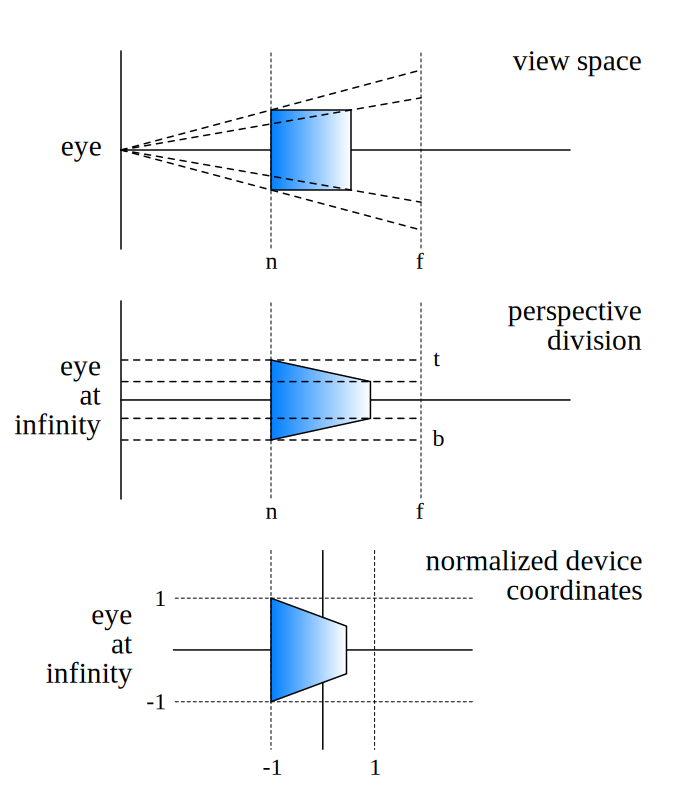
\includegraphics[width=0.8\columnwidth]{./images/view_coordinates_to_ndc.png}
    \caption{Perspective projection from view space to NDC in 2d.}
    \label{img:view_to_ndc}
\end{figure}

\begin{figure}
    \centering
    \includegraphics[width=0.7\columnwidth]{./images/wireframes.png}
    \caption{Different car wireframes used. From left to right Ford Explorer, Volvo V60, Nissan Altima.}
    \label{img:wireframes}
\end{figure}

double column text here. .double column text here. . .
double column text here. . .
double column text here. . .
double column text here. . .lkasj fundingasdf
double column text here. .double column text here. . .
double column text here. . .
double column text here. . .
double column text here. . .lkasj fundingasdf
double column text here. .double column text here. . .
double column text here. . .
double column text here. . .
double column text here. . .lkasj fundingasdf

\begin{wrapfigure}{L}{0.5\columnwidth}
    \centering
    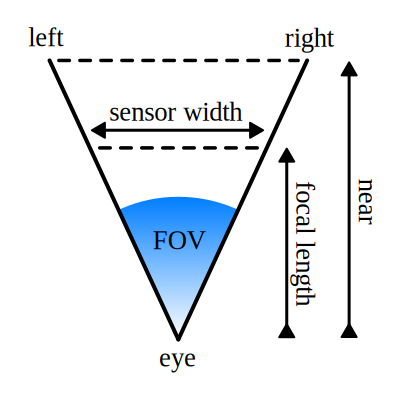
\includegraphics[width=0.45\columnwidth]{./images/focal_lenght_and_field_of_view.png}
    \caption{The sensor width and the focal length are used to calculate the camera's field of view.}
    \label{img:fov}
\end{wrapfigure}

double column text here. .double column text here. . .
double column text here. . .
double column text here. . .
double column text here. . .lkasj fundingasdf
double column text here. .double column text here. . .
double column text here. . .
double column text here. . .
double column text here. . .lkasj fundingasdf

Matrix representation of the standard projection onto the z = 1 plane.
\begin{equation}
    \begin{bmatrix}
        1 & 0 & 0 & 0 \\
        0 & 1 & 0 & 0 \\
        0 & 0 & 1 & 0 \\
        0 & 0 & 1 & 0
    \end{bmatrix}
    \begin{bmatrix}
        x \\
        y \\
        z \\
        1
    \end{bmatrix}
    =
    \begin{bmatrix}
        x \\
        y \\
        z \\
        z
    \end{bmatrix}
    \overset{\text{div z}}{\equiv}
    \begin{bmatrix}
        \frac{x}{z} \\
        \frac{y}{z} \\
        1           \\
    \end{bmatrix}
\end{equation}

\begin{figure*}[htbp]
    \begin{equation} \label{eqn:DLT}
        \begin{bmatrix}
            -c_1 x_1 & -c_1 y_1 & -c_1 z_1 & -c_1   & 0        & 0        & 0        & 0      & x_1 x_{1}' & y_1 x_{1}' & z_1 x_{1}' & x_{1}' \\
            0        & 0        & 0        & 0      & -c_2 x_1 & -c_2 y_1 & -c_2 z_1 & -c_2   & x_1 y_{1}' & y_1 y_{1}' & z_1 y_{1}' & y_{1}' \\
            \vdots   & \vdots   & \vdots   & \vdots & \vdots   & \vdots   & \vdots   & \vdots & \vdots     & \vdots     & \vdots     & \vdots \\
            -c_1 x_n & -c_1 y_n & -c_1 z_n & -c_1   & 0        & 0        & 0        & 0      & x_n x_{n}' & y_n x_{n}' & z_n x_{n}' & x_{n}' \\
            0        & 0        & 0        & 0      & -c_2 x_n & -c_2 y_n & -c_2 z_n & -c_2   & x_n y_{n}' & y_n y_{n}' & z_n y_{n}' & y_{n}' \\
        \end{bmatrix}
        \begin{bmatrix}
            a      \\
            b      \\
            \vdots \\
            k      \\
            l
        \end{bmatrix}
        =
        \begin{bmatrix}
            0      \\
            0      \\
            \vdots \\
            0      \\
            0
        \end{bmatrix}
    \end{equation}
\end{figure*}


The API projection Matrix






To get the screen-space position of a vertex, we multiply it by its Modelview Matrix and API Projection Matrix before doing the projective division.
We have all the parameters except the Model Matrix. $p' = M_{API} M_{Modelview} p$

\begin{equation*}
    \begin{bmatrix}
        x' \\
        y' \\
    \end{bmatrix}
    \overset{\text{div w}}{\equiv}
    \begin{bmatrix}
        c_1 & 0   & 0   & 0   \\
        0   & c_2 & 0   & 0   \\
        0   & 0   & c_3 & c_4 \\
        0   & 0   & 1   & 0
    \end{bmatrix}
    \begin{bmatrix}
        a & b & c & d \\
        e & f & g & h \\
        i & j & k & l \\
        0 & 0 & 0 & 1
    \end{bmatrix}
    \begin{bmatrix}
        x \\
        y \\
        z \\
        1
    \end{bmatrix}
\end{equation*}

If we multiply that out, we get for $x'$ and $y'$:

\begin{gather*}
    x' = \frac{c_1 a x + c_1 b y + c_1 c z + c_1 d}{ix + jy + kz + l} \\
    y' = \frac{c_2 e x + c_2 f y + c_2 g z + c_2 h}{ix + jy + kz + l}
\end{gather*}

We can multiply by the denuminator and solve for 0. Since this holds for every pair of points $(p_{1} , p_{1}'), (p_{2} , p_{2}'), ..., (p_{n}, p_{n}')$ that we track we can create the following system of equation:
\ref{eqn:DLT}


\bibliographystyle{./IEEEtran.bst}
\bibliography{./robot_vision}

\end{document}
